\section{Procedure e protocolli}
\subsection{Protocollo di sviluppo del progetto}
\subsubsection{Utilizzo del ticketing}
Ogni membro del team \textit{Sirius} avrà accesso al sistema di \textit{ticketing}. Le figure che invece potranno assegnare ticket sono le seguenti:

\begin{itemize}
\item Il \textit{Responsabile di Progetto} assegnerà i \textit{ticket} di massima importanza cioè quelli correlati allo sviluppo delle attività necessarie all' avanzamento del progetto;
\item Il \textit{Verificatore} potrà assegnare \textit{ticket} allo scopo di segnalare errori di grave entità rilevati durante l'attività di verifica.
\end{itemize}

Di conseguenza i \textit{ticket} sono suddivisi in due macro-categorie:
\begin{itemize}
\item \textit{Ticket} di pianificazione, i quali rappresentano le attività che devono essere svolte per procedere con l'avanzamento del progetto, sono suddivisi in 4 sotto-categorie:
\begin{itemize}
\item \emph{Documento}: che rappresenta una \textit{task} inerente alla redazione di un documento; 
\item \emph{Codice}: che rappresenta una \textit{task} inerente alla stesura di codice;
\item \emph{Verifica}: che rappresenta una \textit{task} inerente all'attività di verifica di un'attività;
\item \emph{Generali}: che rappresenta \textit{tasks} i cui scopi sono svariati ed in genere non ad alta priorità, come ad esempio la ricerca di un determinato \textit{software}.
\end{itemize}
lo svolgimento dell'insieme di tutti i ticket di una \textit{task-list} non porterà alla conclusione della \textit{task-list} stessa, questo poiché è prevista la possibilità di aggiungere durante l'avanzamento del progetto ulteriori \textit{task}, fino a quando il \textit{responsabile di progetto} non ne dichiarerà la conclusione;
\item Ticket di verifica, contenenti gli errori identificati dai \textit{verificatori} a seguito dell'analisi del lavoro svolto da qualche membro del \textit{team}.
\end{itemize}

Ogni membro del \textit{team} sarà tenuto ad utilizzare la barra di avanzamento di stato del \textit{ticket} fornita dall'interfaccia di \textit{TeamWorkPM}, evitando così superflue norme aggiuntive atte a determinare lo stato del \textit{ticket}.

\subsubsection{Creazione di una milestone}
Il \textit{Responsabile di Progetto} dovrà creare una \textit{milestone}, essa indica la data della revisione a cui il gruppo \gruppo{} intende presentarsi, è possibile visualizzare lo stato di avanzamento che tiene conto del numero di \textit{ticket} completati rispetto al numero di \textit{ticket} complessivi.
Per la creazione di una nuova \textit{milestone} il \textit{Responsabile di Progetto} dovrà seguire i seguenti passi:
\begin{enumerate}
\item Aprire il progetto dall'interfaccia \textit{web} di \textit{TeamWorkPM};
\item Posizionarsi sull'opzione: "\emph{Milestones}" ed accedervi;
\item Cliccare sull'opzione: "\emph{Add a new milestone}".
\end{enumerate}

Completati questi passaggi apparirà il seguente \textit{form\ped{G}} (fig 1) che dovrà essere compilato per concludere la creazione della una \textit{milestone}.
\begin{figure}
\centering
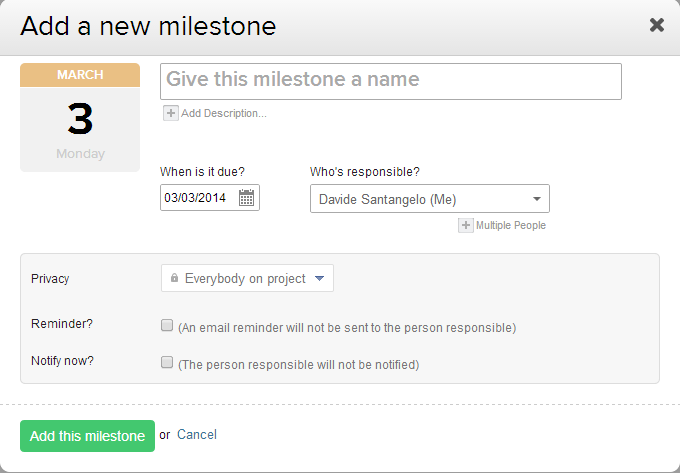
\includegraphics[width=%
\textwidth]{immaginiNDP/Immagine}
\caption[]{Creazione di una milestone.}
\label{fig:Immagine}
\end{figure}

\subsubsection{Procedura di creazione ticket} 
Il \textit{Responsabile di Progetto} dovrà attenersi alla seguente procedura per la creazione di una nuova task-list, ovvero la concretizzazione di un macro-attività e delle sue relative task (ticket). Si ricorda che TeamWorkPM prevede la possibilità di indicare interdipendenze tra task-list.
\begin{enumerate}
\item Dall'interfaccia \textit{web} accedere al progetto \progetto{}, e selezionare dal \textit{menù} principale il comando: \emph{"Task"};
\item Procedere, se necessario, con la creazione di una nuova \textit{task-list} tramite il comando: \emph{"Add task list"};
\item Una volta creata la \textit{task-list} sarà possibile creare i \textit{ticket} (\textit{Task} nel contesto di \textit{TeamWorkPM}) inerenti alla \textit{task-list} scelta.
\end{enumerate}

La struttura di un \textit{ticket} è visualizzabile nella figura 2 di questa sezione.
\begin{figure}
\centering
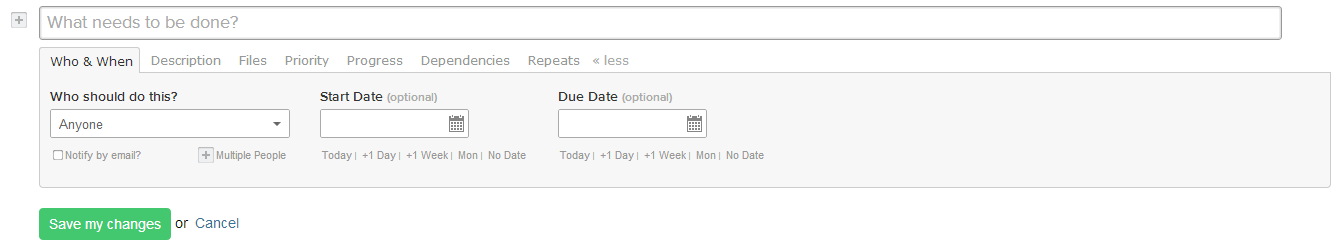
\includegraphics[width=%
\linewidth]{immaginiNDP/creazionetask}
\caption[]{Creazione di un ticket.}
\label{fig:creazionetask}
\end{figure}

Nella task è necessario specificare \textbf{obbligatoriamente}:
\begin{itemize}
\item Il \textbf{Titolo} del \textit{ticket}, dovrà contenere tra parentesi quadre la categoria (per i \textit{ticket} di pianificazione anche la sotto-categoria) di \textit{ticket} di cui si tratta;
\item Il \textbf{Destinatario} del \textit{ticket}, cioè colui a cui è stato assegnato;
\item Le \textbf{Date} di inizio e scadenza del \textit{ticket};
\item Le \textbf{Dipendenze} del \textit{ticket}, che specificano l' eventuale necessità di attendere la terminazione di un insieme di \textit{task} prima di poter svolgere quel determinato compito;
\item Una \textbf{Descrizione} la quale dovrà essere breve e coincisa, ma spiegare efficacemente il lavoro assegnato;
\item La \textbf{Priorità} del \textit{ticket} suddivisa in tre categorie: bassa, media, alta.
\end{itemize}

Compilati i seguenti campi, il \textit{ticket} sarà creato ed inviato regolamentarmene.

\subsubsection{Procedura di terminazione ticket}
Se un \textit{ticket} sarà completato è necessario applicare questa procedura di accertamento:
\begin{enumerate}
\item Il membro del \textit{team} a cui è stato assegnato il \textit{ticket} dovrà spuntare la casella di terminazione su \textit{TeamWorkPM};
\item Durante il controllo giornaliero il \textit{Responsabile di Progetto} controllerà quanto necessario a determinare che il lavoro sia stato effettivamente svolto;
\item Se il lavoro è stato effettivamente svolto, sarà avviato un \textit{ticket} di \emph{Pianificazione} a scopo di verificare il lavoro;
\item Nel caso di irregolare svolgimento del \textit{ticket} o problemi di grave entità, il \textit{Responsabile di Progetto} dovrà applicare la procedura di modifica o riassegnazione del \textit{ticket} presente nel prossimo paragrafo;
\item Nel caso di esito positivo (cioè con regolare svolgimento) il \textit{ticket} sarà concluso ed archiviato, mentre al contempo, qualora fosse necessario, saranno avviati dei \textit{ticket} di \emph{Verifica} per la correzione degli errori non gravi rilevati durante la \textit{Verifica};

\end{enumerate}

\subsubsection{Procedura per la modifica o riassegnazione ticket} 
Durante il suo ciclo di vita un \textit{ticket} per varie ragioni può andare in contro a modifiche, è necessario quindi normare la seguente procedura:
\begin{enumerate}
\item Aprire il progetto dall'interfaccia \textit{web} di \textit{TeamWorkPM};
\item Selezionare il \textit{ticket} di interesse;
\item Selezionare il comando: \emph{"Edit Task"};
\item Aggiungere una descrizione riguardo la modifica effettuata;
\item Avvertire l'interessato che è stata effettuata una modifica inserendo: "(MOD)" sul titolo del \textit{ticket}, e qualora fosse necessario reimpostandone la sua priorità.
\end{enumerate}

\subsection{Protocollo di pianificazione}
Il \textit{responsabile di progetto} per ogni attività indicata nel documento \textit{Piano di Progetto} dovrà creare un nuovo progetto seguendo la procedura qui descritta:

\begin{enumerate}
\item Inserire una milestone\ped{G};
\item Inserire le attività da svolgere;
\item Inserire le rispettive sotto-attività;
\item Calcolare ed inserire i periodi di slack\ped{G} qualora fosse necessario;
\item Creare le risorse;
\item Assegnare le risorse create ad ogni attività;
\item Salvare la baseline\ped{G}.
\end{enumerate}

Sarà decisa a discrezione del \textit{Responsabile di Progetto} per ogni attività la possibilità di assegnare un surplus di ore, queste ore supplementari verranno scelte basandosi sulla criticità dell'attività considerata.

\begin{itemize}
\item Per le attività non critiche non è previsto alcun surplus di ore;
\item Per le attività di media criticità il surplus di ore potrà essere del 15\%;
\item Per le attività di criticità massima il surplus di ore potrà essere del 30\%.
\end{itemize}
\subsection{Protocollo di verifica}
\subsubsection{Tecniche di analisi statica}
L'analisi statica è una tecnica di analisi applicabile sia alla documentazione che al codice e permette di effettuare la verifica di quanto prodotto individuando errori ed anomalie. Essa può essere svolta in due modi diversi ma complementari tra di loro in quanto per utilizzare \textit{inspection} bisogna prima aver effettuato \textit{walkthrough}
\paragraph{Inspection}
Questa tecnica, di analisi statica, consiste nella verifica di sezioni ben definite di un documento o del codice. Questo tipo di controlli per i documenti sono usualmente definiti tramite una lista di controllo (checklist) redatta anticipatamente rispetto all'attività di verifica da intraprendere. Per la verifica dei documenti, la lista di controllo è stata elaborata a seguito di analisi eseguite tramite \textit{walkthrough}, ed evidenziando gli errori più ricorrenti riscontrati. \textit{Inspection} è una strategia rapida in quanto permette l'analisi di alcuni parti ritenute critiche nella checklist senza bisogno di una lettura integrale di documento o di tutto il codice in oggetto.
\paragraph{Walkthrough}
\textit{Walkthrough} è una tecnica di analisi statica che consiste nella lettura critica a largo raggio di tutto il documento. In questa tipologia di analisi il \textit{Verificatore} utilizza molto tempo per la lettura e correzione del documento o codice. Questa tecnica viene di solito utilizzata nella prima parte dello sviluppo di progetti in quanto, la poca esperienza del \textit{Verificatore} non permette un'altro tipo di verifica. Al termine di questo primo set di analisi \textit{walkthrough} viene usualmente definita una lista di controllo che permetta di ricercare in primo luogo gli errori più ricorrenti, e maggiormente riscontrati. \textit{Walkthrough} è un'attività onerosa e collaborativa che richiede l'intervento di più persone per essere efficiente ed efficace
\subsubsection{Tecniche di analisi dinamica}
L'analisi dinamica si applica solamente al prodotto software e consiste nell'esecuzione del codice mediante l'uso di test predisposti per verificarne il funzionamento o rilevare possibili difetti di implementazione eseguendo tutto o solo una parte del codice.
La \textbf{ripetibilità} del test è una caratteristica fondamentale per questo tipo di test, in quanto dichiara che il codice con un certo \textit{input} produce sempre lo stesso \textit{output} su uno specifico ambiente. In questo modo si è in grado di riscontrare problemi e verificare la correttezza del prodotto.
Per questo \gruppo ~ha deciso di definire a priori le seguenti caratteristiche:
\begin{itemize}
\item \textbf{Ambiente}: sistema \textit{hardware} e quello \textit{software} sui quali è stato pianificato l'utilizzo del prodotto, di essi si deve definire uno stato iniziale dal quale poter iniziare ad eseguire i test;
\item \textbf{Specifica di \textit{input}}: definire quali sono gli \textit{input} e quali devono essere gli \textit{output} attesi;
\item \textbf{Procedure}: definire quali devono essere i test ed in che ordine devono essere analizzati i risultati ottenuti.
\end{itemize}
Di seguito sono definiti cinque diversi tipi di test.
\paragraph{Test di unità} 
Per test di unità si intende la verifica di ogni singola unità di prodotto software tramite l'utilizzo di stub\ped{G}, driver\ped{G} e logger\ped{G}. Per unità si intende la più piccola porzione di codice che è utile verificare singolarmente e che viene prodotta da un unico programmatore. Tramite questo tipo di test si vogliono testare i vari le unità per rilevare errori di implementazione da parte dei programmatori.
\paragraph{Test di integrazione}
I test di integrazione prevedono la verifica dei componenti del sistema che vengono aggiunti incrementando il prodotto di origine e si prefigge quindi di analizzare la combinazione di due o più unità software che hanno quindi superato i test di unità. Questa tecnica di verifica serve ad individuare errori residui nella programmazione dei singoli moduli: come modifiche delle interfacce e comportamenti inaspettati di componenti software di parti terze e che pregiudicherebbero la validità del prodotto. Per effettuare tali test può essere necessario l'aggiunta di componenti software fittizie e non ancora implementate al fine di non pregiudicare negativamente l'esito dell'analisi.
\paragraph{Test di sistema}
Consiste nella validazione del sistema attraverso la verifica della copertura di tutti i requisiti obbligatori individuati in \infoAR, e tracciati  grazie allo strumento messo a punto da \gruppo;
\paragraph{Test di regressione}
I test di regressione vengono eseguiti quando si apportano delle modifiche a parte del software e questi consistono nella riesecuzione dei test riguardanti le i componenti che hanno subito modifiche e che precedentemente non erano soggetti ad errori.
Tale operazione viene aiutata dal tracciamento, che permette di individuare e ripetere facilmente i test di unità, integrazione ed eventualmente di sistema che sono stati potenzialmente influenzati dalle modifiche.
\paragraph{Test di accettazione}
Si tratta del collaudo del prodotto software sotto il controllo del proponente. Se il collaudo viene superato in modo positivo, il sistema viene rilasciato e la commessa si conclude.